\chapter{Исследование параметров РТГС на основе $Al_{x}Ga_{1-x}As$}
\section{Исследование парметров ямы}

\subsection{Исследование глубины ямы}
\subsubsection{ВАХ РТГС}
\subsubsection{Прозрачность РТГС}

\subsection{Исследование ширины ямы}
\subsubsection{ВАХ РТГС}
\subsubsection{Прозрачность РТГС}

% % \section{Алгорит моделирования деградации ГС}
% % \begin{figure}[h]
% %   \centering
% %   \includegraphics[width=0.7\linewidth]{assets/AlgDegrVAC}
% %   \caption{Блок схема алгорит моделирования деградации ГС}
% %   \label{img:AlgDegrVAC}
% % \end{figure}
% % \section{Начальные условия}
% \section{Моделирование диффузионного размытия в <<закрытой системе>> $i\!-\!GaAs/i\!-\!Al_{45}Ga_{55}As$}
% \begin{figure}[h]
% 	\centering
%     \includegraphics[width=0.3\textwidth]{DifCloseAlGaAs3D}
%     \caption{Структура}
% \end{figure}
% \begin{figure}[h]
% 	\centering
%     \includegraphics[width=0.8\textwidth]{DifCloseAlGaAs}
%     \caption{Профиль дна зоны проводимости}
% \end{figure}

% \begin{figure}[h]
%   \centering
%   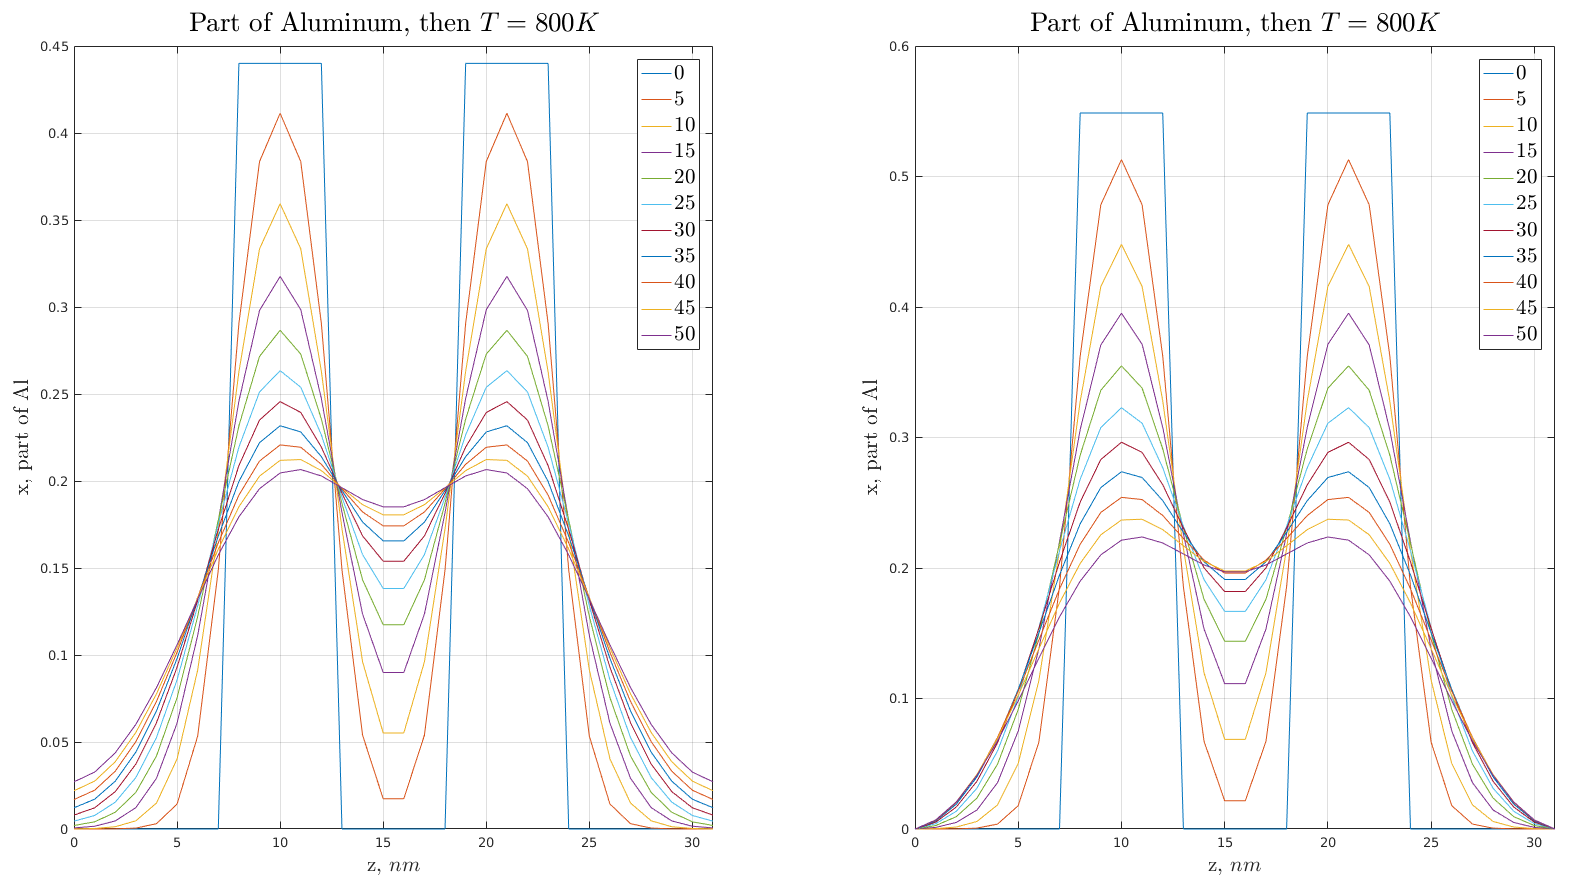
\includegraphics[width=\linewidth]{DCAlGaAs}
%   \caption{Диффузионное размытие}
% \end{figure}

% \begin{figure}[h]
%   \centering
%   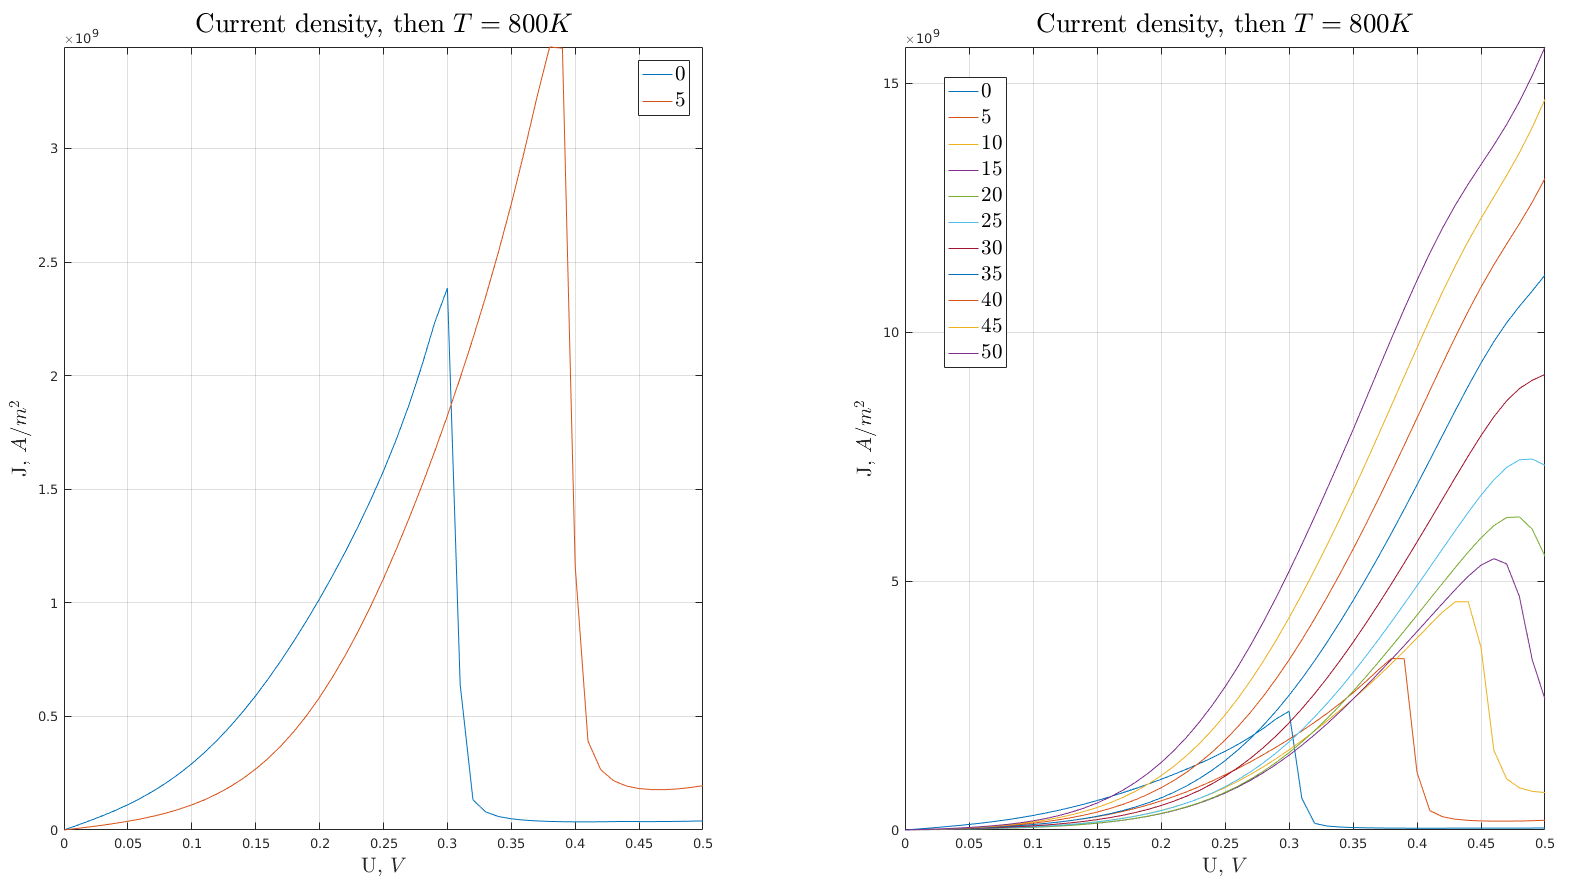
\includegraphics[width=\linewidth]{JDCAlGaAs}
%   \caption{Деградация ВАХ}
% \end{figure}

% \begin{figure}[h]
%   \centering
%   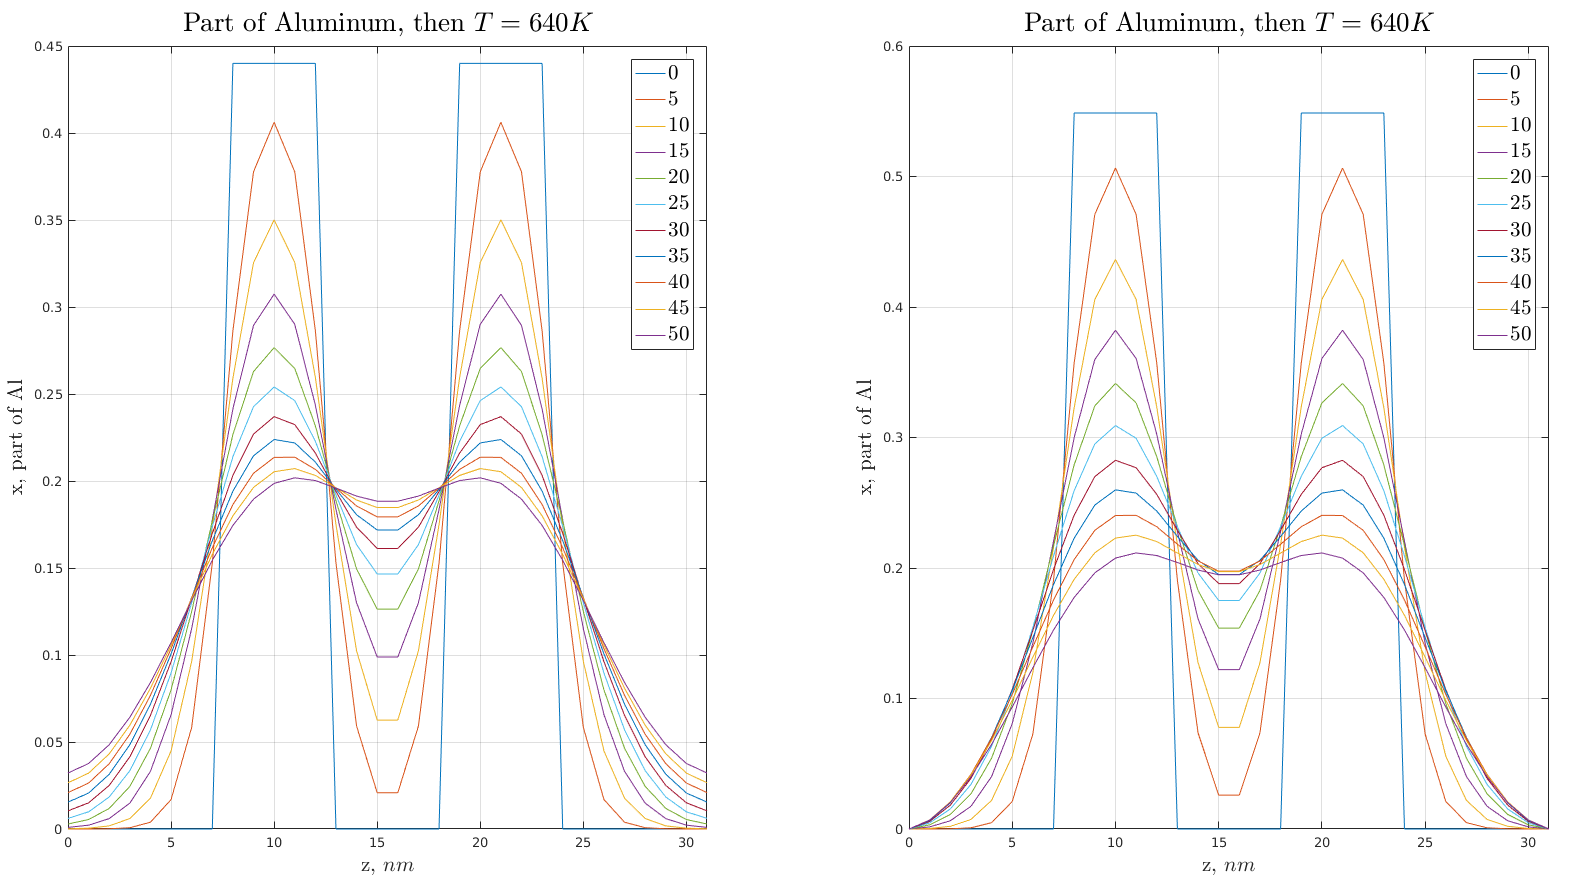
\includegraphics[width=\linewidth]{DCAlGaAsNd}
%   \caption{Диффузионное размытие с учетом примеси, $Nd = 5*10^{15}sm^{-3}$}
% \end{figure}

% \begin{figure}[h]
%   \centering
%   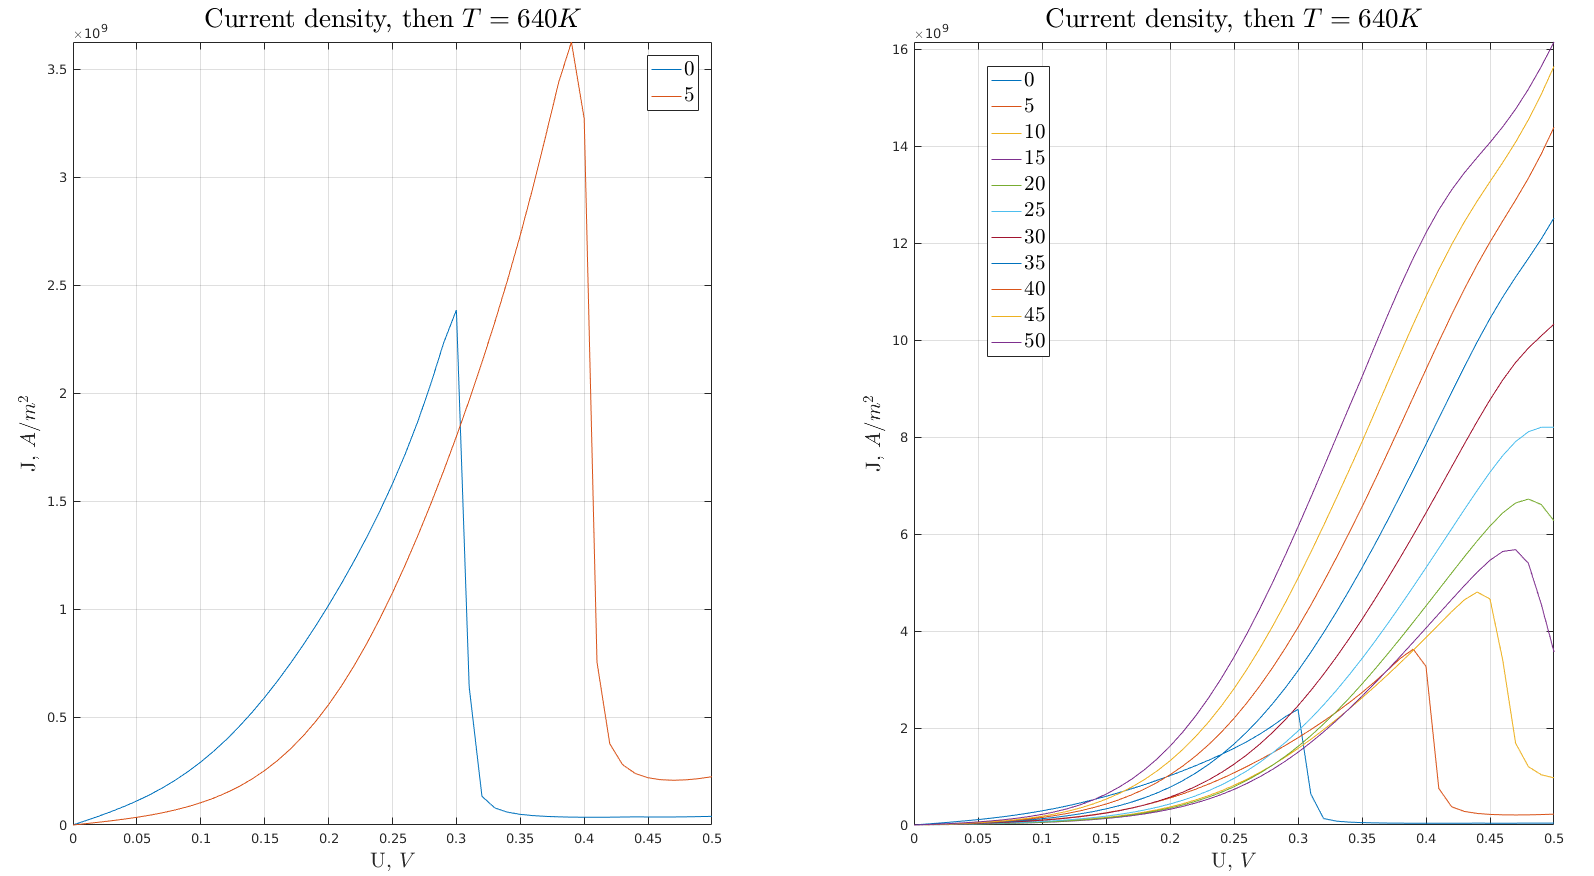
\includegraphics[width=\linewidth]{JDCAlGaAsNd}
%   \caption{Деградация ВАХ с учетом примеси, $Nd = 5*10^{15}sm^{-3}$}
% \end{figure}